%
% management.tex
%
% Copyright The GOLDS-UFSC Contributors.
%
% GOLDS-UFSC Documentation
%
% This work is licensed under the Creative Commons Attribution-ShareAlike 4.0
% International License. To view a copy of this license,
% visit http://creativecommons.org/licenses/by-sa/4.0/.
%

%
% \brief Mission management chapter.
%
% \author Gabriel Mariano Marcelino <gabriel.mm8@gmail.com>
%
% \version 0.2.0
%
% \date 2021/07/15
%

\chapter{Mission Management} \label{ch:management}

This chapter presents the main aspects of the general management of the project, like the mission schedule, product tree, and so on.


\section{Schedule}

The current schedule of the project is available in \autoref{tab:mission-schedule}.

\begin{table}[!h]
    \centering
    \begin{tabular}{cC{1.2cm}C{1.2cm}C{1.2cm}C{1.2cm}C{1.2cm}C{1.2cm}C{1.2cm}C{1.2cm}C{1.2cm}C{1.2cm}}
        \toprule[1.5pt]
        \multirow{4}{*}{\textbf{Activity}} & \multicolumn{8}{c}{\textbf{Month}} \\
                & Nov & Dez & Jan & Feb & Mar & Apr & May & Jun \\
                & 22  & 22  & 23  & 23  & 23  & 23  & 23  & 23  \\
        \midrule
        1       & \fc & \fc &     &     &     &     &     &     \\
        2       & \fc & \fc & \fc & \fc &     &     &     &     \\
        3       & \fc & \fc & \fc &     &     &     &     &     \\
        4       &     &     &     & \fc & \fc &     &     &     \\
        5       &     &     &     &     & \fc &     &     &     \\
        6       &     &     & \fc & \fc &     &     &     &     \\
        7       &     &     &     &     & \fc &     &     &     \\
        8       &     &     &     &     & \fc & \fc &     &     \\
        9       &     &     &     &     &     & \fc & \fc &     \\
        10      &     &     &     &     &     &     & \fc & \fc \\
        11      &     & \fc &     &     &     &     &     &     \\
        12      &     &     & \fc &     &     &     &     &     \\
        % 13      &     &     &     &     &     &     &     &     &     &     & \fc & \fc & \fc & \fc \\
        % 14      &     &     &     &     &     &     &     &     &     &     &     &     & \fc & \fc \\
        \bottomrule[1.5pt]
    \end{tabular}
    \caption{Mission schedule (updated on 2022/10/24).}
    \label{tab:mission-schedule}
\end{table}

Each activity of \autoref{tab:mission-schedule} is described below:

\begin{enumerate}
    \item Integration of the engineering model in SpaceLab UFSC.
    \item Preparation and suitability of the ground segment.
    \item Verification and validation of the engineering model.
    \item Integration and verification with data collection platforms.
    \item Verification and validation tests of Engineering Model compatibility with EMMN in the INPE / CRN in Natal.
    \item Verification and validation of the flight model.
    \item Environmental tests at the Integration and Testing Laboratory (LIT/INPE).
    \item Flight model acceptance and ground segment review.
    \item Ground segment delivery.
    \item Flight model delivery.
    \item Purchase (flight model).
    \item Delivery of purchased items (flight model).
\end{enumerate}

\section{Product Tree}

The product tree of the GOLDS-UFSC mission is the project breakdown into successive levels of hardware and software products (or elements). The product tree of the project can be seen in the diagram of \autoref{fig:product-tree}. As shown, the satellite was divided into eight segments.

\begin{figure}[!ht]
    \begin{center}
        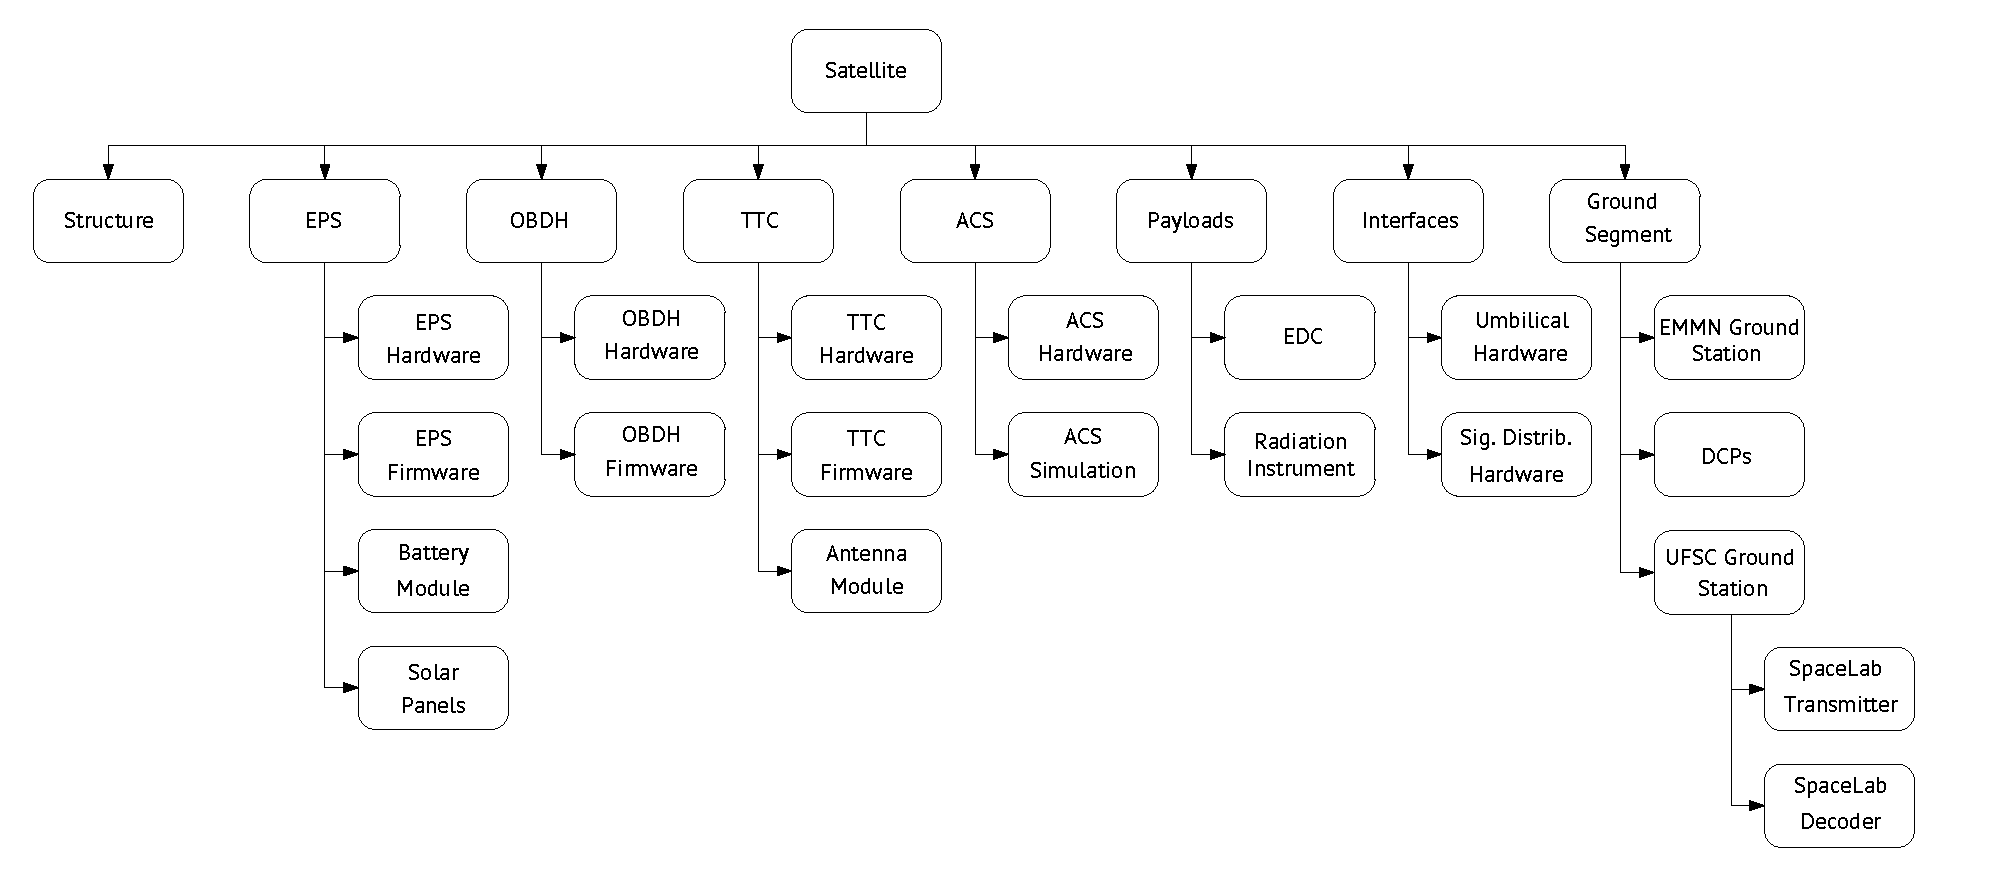
\includegraphics[width=\textwidth]{figures/product-tree.pdf}
        \caption{Product tree of the satellite.}
        \label{fig:product-tree}
    \end{center}
\end{figure}

The responsibility of each segment of the product tree is described next:

\begin{itemize}
    \item \textbf{Structure}: UFSC (COTS\nomenclature{\textbf{COTS}}{\textit{Commercial Off-The-Shelf}.}).
    \item \textbf{EPS}: UFSC (developed in-house, with COTS solar panels).
    \item \textbf{OBDH}: UFSC (developed in-house).
    \item \textbf{TTC}: UFSC (developed in-house).
    \item \textbf{ACS}: UFSC (developed in-house).
    \item \textbf{Payload EDC}: INPE
    \item \textbf{Radiation instrument}: UFSC (developed in-house).
    \item \textbf{Interfaces}: UFSC (developed in-house).
    \item \textbf{Ground segment}:
    \begin{itemize}
        \item \textbf{EMMN ground station}: INPE
        \item \textbf{DCPs}: INPE/SINDA and other institutions
        \item \textbf{UFSC ground station}: UFSC
    \end{itemize}
\end{itemize}

\subsection{Work Breakdown Structure}

The Work Breakdown Structure (WBS\nomenclature{\textbf{WBS}}{\textit{Work Breakdown Structure.}}) is presented as a diagram in \autoref{fig:wbs}. The WBS is divided into work packages (WP\nomenclature{\textbf{WP}}{\textit{Work Package.}}) as can be seen in the diagram. The description of each WP is detailed below.

\begin{figure}[!ht]
    \begin{center}
        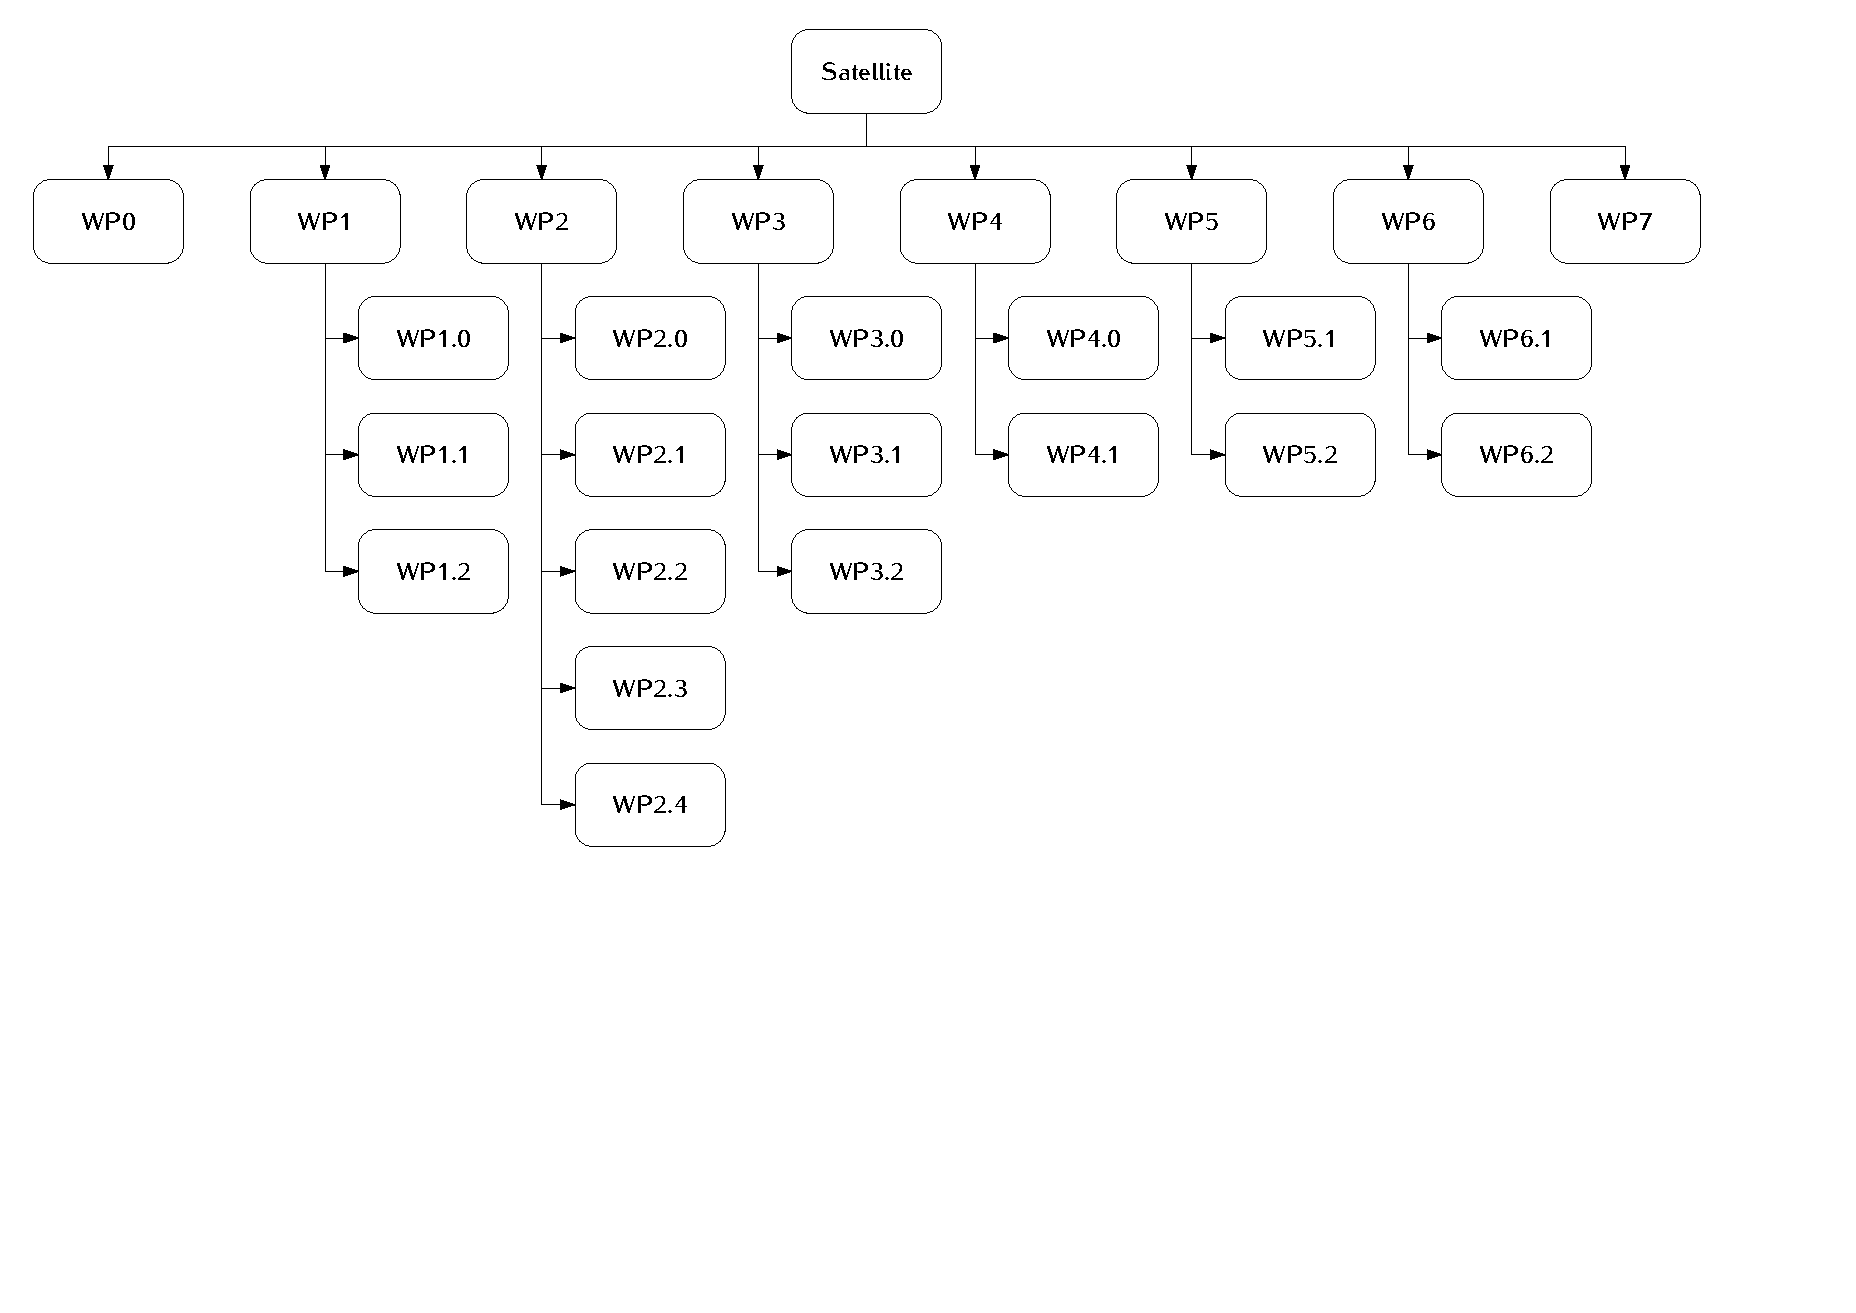
\includegraphics[width=\textwidth]{figures/wbs.pdf}
        \caption{WBS diagram.}
        \label{fig:wbs}
    \end{center}
\end{figure}

\begin{itemize}
    \item \textbf{WP0}: Management and preparation.
    \item \textbf{WP1}: Architecture study and specification.
        \begin{itemize}
            \item \textbf{WP1.0}: Operation scenario definition.
            \item \textbf{WP1.1}: Architecture definition.
            \item \textbf{WP1.2}: Requirements definition.
        \end{itemize}
    \item \textbf{WP2}: Engineering and flight models definition
        \begin{itemize}
            \item \textbf{WP2.0}: Application design.
            \item \textbf{WP2.1}: Platform design.
            \item \textbf{WP2.2}: Application implementation.
            \item \textbf{WP2.3}: Platform implementation.
            \item \textbf{WP2.4}: Decoder implementation (EGSE).
        \end{itemize}
    \item \textbf{WP3}: Engineering model integration.
        \begin{itemize}
            \item \textbf{WP3.0}: Subsystems integration and tests.
            \item \textbf{WP3.1}: Engineering model satellite integration.
            \item \textbf{WP3.2}: Integration and tests with decoder.
        \end{itemize}
    \item \textbf{WP4}: Engineering model validation.
        \begin{itemize}
            \item \textbf{WP4.0}: Validation scenarios specification.
            \item \textbf{WP4.1}: Project validation.
        \end{itemize}
    \item \textbf{WP5}: Fligth model integration.
        \begin{itemize}
            \item \textbf{WP5.0}: Subsystems integration and tests.
            \item \textbf{WP5.1}: Fligth model satellite integration.
        \end{itemize}
    \item \textbf{WP6}: Fligth model validation.
        \begin{itemize}
            \item \textbf{WP6.0}: Validation scenarios specification.
            \item \textbf{WP6.1}: Project validation.
        \end{itemize}
    \item \textbf{WP7}: Evaluation and dissemination.
\end{itemize}


\section{Risk Management}

A risk is an event that threatens the project's success, even if partially. Therefore, this plan aims to help identifying adverse events at an early stage, handle them, and mitigate.

The development of this project will be based on a qualitative risk analysis standard. This depends on crossing two metrics: the probability of risk occurrence and the impact of risk occurrence. \autoref{likelihood} shows definitions of the probability of occurrence categorization.

% Please add the following required packages to your document preamble:
% \usepackage[table,xcdraw]{xcolor}
% If you use beamer only pass "xcolor=table" option, i.e. \documentclass[xcolor=table]{beamer}
\begin{table}[H]
    \centering
    \begin{tabular}{ll}
    \toprule[1.5pt]
    \textbf{Likelihood} &  \textbf{Likelihood of occurrence} \\
    \midrule
    Expected   & Almost certain occurrence. Very likely event to occur. \\
    Probable   & \begin{tabular}[c]{@{}l@{}}Occurs frequently, relatively recurrent observations. \\ Event with considerable chances of occurring.\end{tabular} \\
    Improbable & \begin{tabular}[c]{@{}l@{}}Occurs occasionally, it is not a rare event. Event with \\ a significant but small chance of occurring.\end{tabular} \\
    Rare       & \begin{tabular}[c]{@{}l@{}}Occurs rarely, rare observations. Very unlikely \\ event to occur.\end{tabular} \\
    Very rare  & \begin{tabular}[c]{@{}l@{}}It almost never occurs, very rare occurrences, or \\ never occurred. An almost impossible event to occur.\end{tabular} \\
    \bottomrule[1.5pt]
    \end{tabular}
    \caption{Likelihood categorization.}
    \label{likelihood}
\end{table}

Five levels of impact define the occurrence impact metric:

\begin{itemize}
    \item \textbf{5 (Catastrophic):} In general, these are risks that, if materialized, make the Subject or Activity unfeasible or end. Some examples of the description by feature:
        \begin{itemize}
           \item  \textit{Financial Resources:} Significant increase in expenses that makes the continuation of the project or activity unfeasible or causes its termination;
           \item  \textit{Material Resources:} loss of materials that makes the continuation of the project or activity unfeasible or causes its termination;
           \item  \textit{Temporal Resources:} delay that makes the continuation of the project or activity unfeasible or causes its termination;
           \item  \textit{Human Resources:} Death of one or more people. Evasion of more than 95\% of those involved; and 
           \item  \textit{Organizational Image Resources:} Loss of total institutional credibility.
        \end{itemize}
    \item \textbf{4 (Critical):} Overall, these are risks that, if materialized, make it very difficult to complete or progress the Subject/Activity and may raise considerations of finishing the Subject or Activity. Some examples of the description by resource:
    \begin{itemize}
       \item \textit{ Financial Resources:} Increase of over 50\% in expenses;
       \item  \textit{Material Resources:} Material loss that cannot be replaced in a timely manner and that causes a significant loss of permanent performance of the system;
       \item  \textit{Temporal Resources:} delay of more than 80\% in the estimated time in the conclusion of the Subject/Activity;
       \item  \textit{Human Resources: }Permanent disability of one or more people. Evasion between 70\% and 95\% of those involved; and
       \item  \textit{Organizational Image Resources:} Very strong loss of institutional credibility.
    \end{itemize}
    \item \textbf{3 (Major):} Overall, these are risks that, if materialized, make it difficult to complete or progress the Subject/Activity but do not usually raise considerations about ending the Subject or Activity. Some examples of the description by resource:
    \begin{itemize}
       \item  \textit{Financial Resources:} Increase in subject/activity expenses between 15\% and 50\%;
       \item  \textit{Material Resources:} Material loss capable of being replaced in a timely manner, but causing significant temporary system loss;
       \item  \textit{Temporal Resources: }delay between 40\% and 80\% in the estimated time in the conclusion of the Subject/Activity;
       \item  \textit{Human Resources: }Temporary disability of one or more people. Evasion between 40\% and 70\% of those involved; and
       \item  \textit{Organizational Image Resources:} Loss of significant institutional credibility.
    \end{itemize}
    \item \textbf{2 (Minor):} Overall, these are risks that, if materialized, significantly hamper the completion or progress of the Subject/Activity, but definitely do not raise the consideration of termination. Some examples of the description by feature:
    \begin{itemize}
       \item  \textit{Financial Resources: }Increase in subject/activity expenses between 5\% and 15\%;
       \item  \textit{Material Resources: }Material loss capable of being replaced in a timely manner and causing a temporary loss of system performance;
       \item  \textit{Temporal Resources:} delay between 10\% and 20\% in the estimated time for completion of the Subject/Activity;
       \item \textit{ Human Resources:} Minor injuries to one or more people. Evasion between 25\% and 40\% of those involved; and
       \item  \textit{Organizational Image Resources:} Some loss of institutional credibility.
    \end{itemize}
    \item \textbf{1 (Insignificant):} Overall, these are risks that, if materialized, make it a little difficult to complete or progress the Subject/Activity. Some examples of the description by resource:
    \begin{itemize}
         \item  \textit{Financial Resources:} Increase in subject/activity expenses by up to 5\%;
         \item  \textit{Material Resources:} Loss of material that does not cause temporary loss of performance;
         \item  \textit{Temporal Resources:} delay of up to 10\% in the estimated time in the conclusion of the Subject/Activity;
         \item  \textit{Human Resources:} Minor injuries to one or more people. Evasion of less than 25\% of those involved; and
         \item  \textit{Organizational Image Resources:} Little loss of institutional credibility.
    \end{itemize}
\end{itemize}

\subsection{Risks identification}

The identified risks are displayed in \autoref{risk_ID}, classified by context (mission or system), likelihood (Very Rare-Expected), and by level of impact (1-5).

\begin{table}[H]
    \centering
    \begin{tabular}{lL{0.45\textwidth}ccc}
    \toprule[1.5pt]
    \textbf{ID} & \textbf{Risk} & \textbf{Context} & \textbf{Likelihood} & \textbf{Impact} \\
    \midrule
    RSK-1 & Unable to obtain additional financial resources to complete the mission & Mission & Improbable & 5 \\
    RSK-2 & Lack of components on the market & Mission & Probable & 2 \\
    RSK-3 & High turnover of the development team & Mission  & Improbable & 2 \\
    RSK-4 & Significant rise in the dollar (may not have enough resources to acquire systems) & Mission & Probable & 3 \\
    RSK-5 & Satellite commissioning failure & Mission & Improbable & 5 \\
    RSK-6 & Satellite does not survive launch & Mission & Rare & 5 \\
    RSK-7 & Ground Station failure & Mission & Improbable & 5 \\
    RSK-8 & LIT not available for satellite qualification tests & Mission  & Improbable & 2 \\
    RSK-9 & Operational licensing not available on launch time & Mission  & Improbable & 3 \\
    RSK-10 & EPS Software operation failure & System & Improbable & 5 \\
    RSK-11 & OBDH software operation failure & System & Improbable & 5 \\
    RSK-12 & Radiation instrument operation failure & System  & Improbable & 1 \\
    RSK-13 & GSE software operation failure & System  & Improbable & 4 \\
    RSK-14 & EDC does not comply with requirements & System & Rare & 4  \\
    RSK-15 & Materials resources not sufficient for preliminary tests & System & Probable & 2 \\
    RSK-16 & Fail on vibration tests impacting on delays & System  & Rare & 3 \\
    RSK-17 & Non compliant metrological requirements impacting on delays & System & Probable & 2 \\
    RSK-18 & Kill switch mechanism fail, and satellite does not power on & System & Very rare & 5 \\
    RSK-19 & COTS systems not available in market & System & Rare & 3 \\
    \bottomrule[1.5pt]
    \end{tabular}
    \caption{Mission and space systems risks.}
    \label{risk_ID}
\end{table}